% Options for packages loaded elsewhere
\PassOptionsToPackage{unicode}{hyperref}
\PassOptionsToPackage{hyphens}{url}
%
\documentclass[
  8pt,
  ignorenonframetext,
]{beamer}
\usepackage{pgfpages}
\setbeamertemplate{caption}[numbered]
\setbeamertemplate{caption label separator}{: }
\setbeamercolor{caption name}{fg=normal text.fg}
\beamertemplatenavigationsymbolsempty
% Prevent slide breaks in the middle of a paragraph
\widowpenalties 1 10000
\raggedbottom
\setbeamertemplate{part page}{
  \centering
  \begin{beamercolorbox}[sep=16pt,center]{part title}
    \usebeamerfont{part title}\insertpart\par
  \end{beamercolorbox}
}
\setbeamertemplate{section page}{
  \centering
  \begin{beamercolorbox}[sep=12pt,center]{part title}
    \usebeamerfont{section title}\insertsection\par
  \end{beamercolorbox}
}
\setbeamertemplate{subsection page}{
  \centering
  \begin{beamercolorbox}[sep=8pt,center]{part title}
    \usebeamerfont{subsection title}\insertsubsection\par
  \end{beamercolorbox}
}
\AtBeginPart{
  \frame{\partpage}
}
\AtBeginSection{
  \ifbibliography
  \else
    \frame{\sectionpage}
  \fi
}
\AtBeginSubsection{
  \frame{\subsectionpage}
}
\usepackage{amsmath,amssymb}
\usepackage{lmodern}
\usepackage{iftex}
\ifPDFTeX
  \usepackage[T1]{fontenc}
  \usepackage[utf8]{inputenc}
  \usepackage{textcomp} % provide euro and other symbols
\else % if luatex or xetex
  \usepackage{unicode-math}
  \defaultfontfeatures{Scale=MatchLowercase}
  \defaultfontfeatures[\rmfamily]{Ligatures=TeX,Scale=1}
\fi
% Use upquote if available, for straight quotes in verbatim environments
\IfFileExists{upquote.sty}{\usepackage{upquote}}{}
\IfFileExists{microtype.sty}{% use microtype if available
  \usepackage[]{microtype}
  \UseMicrotypeSet[protrusion]{basicmath} % disable protrusion for tt fonts
}{}
\makeatletter
\@ifundefined{KOMAClassName}{% if non-KOMA class
  \IfFileExists{parskip.sty}{%
    \usepackage{parskip}
  }{% else
    \setlength{\parindent}{0pt}
    \setlength{\parskip}{6pt plus 2pt minus 1pt}}
}{% if KOMA class
  \KOMAoptions{parskip=half}}
\makeatother
\usepackage{xcolor}
\newif\ifbibliography
\usepackage{color}
\usepackage{fancyvrb}
\newcommand{\VerbBar}{|}
\newcommand{\VERB}{\Verb[commandchars=\\\{\}]}
\DefineVerbatimEnvironment{Highlighting}{Verbatim}{commandchars=\\\{\}}
% Add ',fontsize=\small' for more characters per line
\usepackage{framed}
\definecolor{shadecolor}{RGB}{248,248,248}
\newenvironment{Shaded}{\begin{snugshade}}{\end{snugshade}}
\newcommand{\AlertTok}[1]{\textcolor[rgb]{0.94,0.16,0.16}{#1}}
\newcommand{\AnnotationTok}[1]{\textcolor[rgb]{0.56,0.35,0.01}{\textbf{\textit{#1}}}}
\newcommand{\AttributeTok}[1]{\textcolor[rgb]{0.77,0.63,0.00}{#1}}
\newcommand{\BaseNTok}[1]{\textcolor[rgb]{0.00,0.00,0.81}{#1}}
\newcommand{\BuiltInTok}[1]{#1}
\newcommand{\CharTok}[1]{\textcolor[rgb]{0.31,0.60,0.02}{#1}}
\newcommand{\CommentTok}[1]{\textcolor[rgb]{0.56,0.35,0.01}{\textit{#1}}}
\newcommand{\CommentVarTok}[1]{\textcolor[rgb]{0.56,0.35,0.01}{\textbf{\textit{#1}}}}
\newcommand{\ConstantTok}[1]{\textcolor[rgb]{0.00,0.00,0.00}{#1}}
\newcommand{\ControlFlowTok}[1]{\textcolor[rgb]{0.13,0.29,0.53}{\textbf{#1}}}
\newcommand{\DataTypeTok}[1]{\textcolor[rgb]{0.13,0.29,0.53}{#1}}
\newcommand{\DecValTok}[1]{\textcolor[rgb]{0.00,0.00,0.81}{#1}}
\newcommand{\DocumentationTok}[1]{\textcolor[rgb]{0.56,0.35,0.01}{\textbf{\textit{#1}}}}
\newcommand{\ErrorTok}[1]{\textcolor[rgb]{0.64,0.00,0.00}{\textbf{#1}}}
\newcommand{\ExtensionTok}[1]{#1}
\newcommand{\FloatTok}[1]{\textcolor[rgb]{0.00,0.00,0.81}{#1}}
\newcommand{\FunctionTok}[1]{\textcolor[rgb]{0.00,0.00,0.00}{#1}}
\newcommand{\ImportTok}[1]{#1}
\newcommand{\InformationTok}[1]{\textcolor[rgb]{0.56,0.35,0.01}{\textbf{\textit{#1}}}}
\newcommand{\KeywordTok}[1]{\textcolor[rgb]{0.13,0.29,0.53}{\textbf{#1}}}
\newcommand{\NormalTok}[1]{#1}
\newcommand{\OperatorTok}[1]{\textcolor[rgb]{0.81,0.36,0.00}{\textbf{#1}}}
\newcommand{\OtherTok}[1]{\textcolor[rgb]{0.56,0.35,0.01}{#1}}
\newcommand{\PreprocessorTok}[1]{\textcolor[rgb]{0.56,0.35,0.01}{\textit{#1}}}
\newcommand{\RegionMarkerTok}[1]{#1}
\newcommand{\SpecialCharTok}[1]{\textcolor[rgb]{0.00,0.00,0.00}{#1}}
\newcommand{\SpecialStringTok}[1]{\textcolor[rgb]{0.31,0.60,0.02}{#1}}
\newcommand{\StringTok}[1]{\textcolor[rgb]{0.31,0.60,0.02}{#1}}
\newcommand{\VariableTok}[1]{\textcolor[rgb]{0.00,0.00,0.00}{#1}}
\newcommand{\VerbatimStringTok}[1]{\textcolor[rgb]{0.31,0.60,0.02}{#1}}
\newcommand{\WarningTok}[1]{\textcolor[rgb]{0.56,0.35,0.01}{\textbf{\textit{#1}}}}
\setlength{\emergencystretch}{3em} % prevent overfull lines
\providecommand{\tightlist}{%
  \setlength{\itemsep}{0pt}\setlength{\parskip}{0pt}}
\setcounter{secnumdepth}{-\maxdimen} % remove section numbering
\newlength{\cslhangindent}
\setlength{\cslhangindent}{1.5em}
\newlength{\csllabelwidth}
\setlength{\csllabelwidth}{3em}
\newlength{\cslentryspacingunit} % times entry-spacing
\setlength{\cslentryspacingunit}{\parskip}
\newenvironment{CSLReferences}[2] % #1 hanging-ident, #2 entry spacing
 {% don't indent paragraphs
  \setlength{\parindent}{0pt}
  % turn on hanging indent if param 1 is 1
  \ifodd #1
  \let\oldpar\par
  \def\par{\hangindent=\cslhangindent\oldpar}
  \fi
  % set entry spacing
  \setlength{\parskip}{#2\cslentryspacingunit}
 }%
 {}
\usepackage{calc}
\newcommand{\CSLBlock}[1]{#1\hfill\break}
\newcommand{\CSLLeftMargin}[1]{\parbox[t]{\csllabelwidth}{#1}}
\newcommand{\CSLRightInline}[1]{\parbox[t]{\linewidth - \csllabelwidth}{#1}\break}
\newcommand{\CSLIndent}[1]{\hspace{\cslhangindent}#1}
% type setting
% ------------------------------------------------------------------------------
\usepackage[german]{babel}     

% fonts
% ------------------------------------------------------------------------------
\usefonttheme{professionalfonts}

% slide title and horizontal line
% ------------------------------------------------------------------------------
\setbeamertemplate{frametitle}{%
    \vskip-30pt \color{black}\large%
    \begin{minipage}[b][23pt]{120mm}%
    \flushleft\insertframetitle%
    \end{minipage}%
}

\setbeamertemplate{headline}										
{
\vskip10pt\hfill\hspace{3.5mm} 										 
\vskip15pt\color{black}\rule{\textwidth}{0.4pt} 					 
}

% slide number
% ---------------------------------------------------------------
\setbeamertemplate{navigation symbols}{}
\setbeamertemplate{footline}
{
\vskip5pt
\vskip2pt
\makebox[123mm]{\hspace{7.5mm}
\hfill Multivariate Datenanalyse $\vert$ 
\copyright $ $ 2023 Dirk Ostwald CC BY-SA 4.0 $\vert$ 
Folie \insertframenumber}
\vskip4pt
}

% block color scheme
% ------------------------------------------------------------------------------
% colors
\definecolor{white}{RGB}{255,255,255}
\definecolor{grey}{RGB}{235,235,235}
\definecolor{lightgrey}{RGB}{245,245,245}
\definecolor{LightBlue}{RGB}{220,220,255}
\definecolor{darkblue}{RGB}{51, 51, 153}

% definitions and theorems
\setbeamercolor{block title}{fg = black, bg = grey}
\setbeamercolor{block body}{fg = black, bg = lightgrey}

% general line spacing 
% ------------------------------------------------------------------------------
\linespread{1.3}

% local line spacing
% ------------------------------------------------------------------------------
\usepackage{setspace}

% colors
% -----------------------------------------------------------------------------
\usepackage{color}

% justified text
% ------------------------------------------------------------------------------
\usepackage{ragged2e}
\usepackage{etoolbox}
\apptocmd{\frame}{}{\justifying}{}

% bullet point lists
% -----------------------------------------------------------------------------
\setbeamertemplate{itemize item}[circle]
\setbeamertemplate{itemize subitem}[circle]
\setbeamertemplate{itemize subsubitem}[circle]
\setbeamercolor{itemize item}{fg = black}
\setbeamercolor{itemize subitem}{fg = black}
\setbeamercolor{itemize subsubitem}{fg = black}
\setbeamercolor{enumerate item}{fg = black}
\setbeamercolor{enumerate subitem}{fg = black}
\setbeamercolor{enumerate subsubitem}{fg = black}
\setbeamerfont{itemize/enumerate body}{}
\setbeamerfont{itemize/enumerate subbody}{size = \normalsize}
\setbeamerfont{itemize/enumerate subsubbody}{size = \normalsize}

% color links
% ------------------------------------------------------------------------------
\usepackage{hyperref}
\definecolor{urls}{RGB}{204,0,0}
\hypersetup{colorlinks, citecolor = darkblue, urlcolor = urls}


% additional math commands
% ------------------------------------------------------------------------------
\usepackage{bm}                               % bold math symbols
\usepackage{mathtools}                        % pmatrix* environment
\newcommand{\niton}{\not\owns}                % reverse not in

% text highlighting
% ------------------------------------------------------------------------------
\usepackage{soul}
\makeatletter
\let\HL\hl
\renewcommand\hl{%
  \let\set@color\beamerorig@set@color
  \let\reset@color\beamerorig@reset@color
  \HL}
\makeatother

% equation highlighting
% -----------------------------------------------------------------------------
\newcommand{\highlight}[2][yellow]{\mathchoice%
  {\colorbox{#1}{$\displaystyle#2$}}%
  {\colorbox{#1}{$\textstyle#2$}}%
  {\colorbox{#1}{$\scriptstyle#2$}}%
  {\colorbox{#1}{$\scriptscriptstyle#2$}}}%

% additional mathematical operators
% ------------------------------------------------------------------------------
\DeclareMathOperator*{\argmax}{arg\,max}
\DeclareMathOperator*{\argmin}{arg\,min}

\ifLuaTeX
  \usepackage{selnolig}  % disable illegal ligatures
\fi
\IfFileExists{bookmark.sty}{\usepackage{bookmark}}{\usepackage{hyperref}}
\IfFileExists{xurl.sty}{\usepackage{xurl}}{} % add URL line breaks if available
\urlstyle{same} % disable monospaced font for URLs
\hypersetup{
  hidelinks,
  pdfcreator={LaTeX via pandoc}}

\author{}
\date{\vspace{-2.5em}}

\begin{document}

\begin{frame}[plain]{}
\protect\hypertarget{section}{}
\center

\begin{center}
\includegraphics[width=0.2\linewidth]{4_Abbildungen/mvda_4_otto} \end{center}

\vspace{2mm}

\Huge

Multivariate Datenanalyse \vspace{6mm}

\large

MSc Psychologie WiSe 2021/22

\vspace{6mm}
\large

Prof.~Dr.~Dirk Ostwald
\end{frame}

\begin{frame}[plain]{}
\protect\hypertarget{section-1}{}
\vfill
\center
\huge

\textcolor{black}{(4) Eigenanalyse} \vfill
\end{frame}

\begin{frame}{}
\protect\hypertarget{section-2}{}
\vfill
\setstretch{2.5}
\Large

Eigenvektoren und Eigenwerte

Orthonormalzerlegung

Singulärwertzerlegung

Vektorkoordinatentransformation

Selbstkontrollfragen \vfill 
\end{frame}

\begin{frame}{}
\protect\hypertarget{section-3}{}
\vfill
\setstretch{2.5}
\Large

\textbf{Eigenvektoren und Eigenwerte}

Orthonormalzerlegung

Singulärwertzerlegung

Vektorkoordinatentransformation

Selbstkontrollfragen \vfill 
\end{frame}

\begin{frame}{Eigenvektoren und Eigenwerte}
\protect\hypertarget{eigenvektoren-und-eigenwerte}{}
\small
\begin{definition}[Eigenvektor, Eigenwert]
$A \in \mathbb{R}^{m \times m}$ sei eine quadratische Matrix. Dann heißt jeder
Vektor $v \in \mathbb{R}^m, v \neq 0$, für den gilt, dass
\begin{equation}
Av  = \lambda v
\end{equation}
mit $\lambda \in \mathbb{R}$ ein \textit{Eigenvektor} von $A$. $\lambda$
heißt zugehöriger \textit{Eigenwert} von $A$.
\end{definition}

\small

Bemerkungen

\begin{itemize}
\tightlist
\item
  Ein Eigenvektor \(v\) von \(A\) wird durch \(A\) mit einem Faktor
  \(\lambda\) verlängert.
\item
  Jeder Eigenvektor hat einen zugehörigen Eigenwert.
\item
  Die Eigenwerte verschiedener Eigenvektor können identisch sein.
\end{itemize}
\end{frame}

\begin{frame}{Eigenvektoren und Eigenwerte}
\protect\hypertarget{eigenvektoren-und-eigenwerte-1}{}
\small
\begin{theorem}[Multiplikativität von Eigenvektoren]
\justifying
\normalfont
$A \in \mathbb{R}^{m \times m}$ sei eine quadratische Matrix. Wenn $v \in \mathbb{R}^m$
Eigenvektor von $A$ mit Eigenwert $\lambda \in \mathbb{R}$ ist, dann ist auch $av \in \mathbb{R}^m $
mit $a \in \mathbb{R}$ Eigenvektor von $A$ und zwar mit Eigenwert $a\lambda \in \mathbb{R}$.
\end{theorem}

\footnotesize

\underline{Beweis}

Es gilt \begin{equation}
Av = \lambda v \Leftrightarrow a(Av) = a(\lambda)v \Leftrightarrow A(av) = (a\lambda)v
\end{equation} Also ist \(av\) ein Eigenvektor von \(A\) mit Eigenwert
\(a\lambda\).

\(\hfill\Box\)

\small

\textbf{Konvention}

Wir betrachten im Folgenden nur Eigenvektoren mit \(\Vert v \Vert = 1\).
\end{frame}

\begin{frame}[t]{Eigenvektoren und Eigenwerte}
\protect\hypertarget{eigenvektoren-und-eigenwerte-2}{}
\vspace{1mm}

\textcolor{darkblue}{Visualisierung eines Eigenvektors} \footnotesize
\center

Für \(A := \begin{pmatrix} 2 & 1 \\ 1 & 2 \end{pmatrix}\) ist
\(v := \frac{1}{\sqrt{2}} \begin{pmatrix} 1 \\ 1 \end{pmatrix}\)
Eigenvektor zum Eigenwert
\(\lambda = 3, w := \begin{pmatrix} 1 \\ 0 \end{pmatrix}\) ist kein
Eigenvektor.

\begin{center}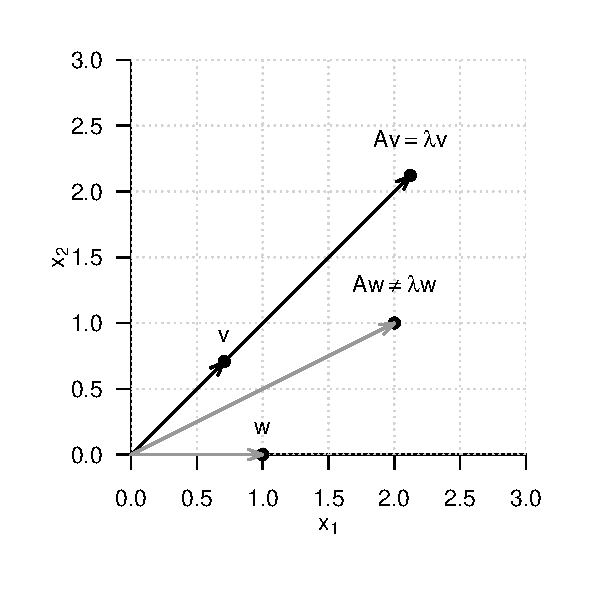
\includegraphics[width=0.55\linewidth]{4_Abbildungen/mvda_4_eigenvektor} \end{center}
\end{frame}

\begin{frame}[fragile]{Eigenvektoren und Eigenwerte}
\protect\hypertarget{eigenvektoren-und-eigenwerte-3}{}
\small
\begin{theorem}[Bestimmung von Eigenwerten und Eigenvektoren]
\normalfont
\justifying
$A \in \mathbb{R}^{m \times m}$ sei eine quadratische Matrix. Dann ergeben sich
die Eigenwerte von $A$ als die Nullstellen des \textit{charakteristischen Polynoms}
\begin{equation}
\chi_A(\lambda) := \det(A - \lambda I_m).
\end{equation}
von $A$. Weiterhin seien $\lambda_i^*, i = 1,2,...$ die auf diese Weise bestimmten
Eigenwerte von $A$. Die entsprechenden Eigenvektoren $v_i, i = 1,2,...$ von $A$
können dann durch Lösen der linearen Gleichungssysteme
\begin{equation}
(A - \lambda_i^* I_m)v_i = 0_m \mbox{ für } i = 1,2,...
\end{equation}
bestimmt werden.
\end{theorem}

\footnotesize

Bemerkungen

\begin{itemize}
\tightlist
\item
  Für kleine Matrizen mit \(m \le 3\) können Eigenwerte und
  Eigenvektoren manuell bestimmt werden.
\item
  Bei großen Matrizen werden Eigenwerte und Eigenvektor im Allgemeinen
  numerisch bestimmt.
\item
  R's \texttt{eigen()}, Scipy's \texttt{linalg.eig()}, Matlab's
  \texttt{eig()}.
\end{itemize}
\end{frame}

\begin{frame}{Eigenvektoren und Eigenwerte}
\protect\hypertarget{eigenvektoren-und-eigenwerte-4}{}
\setstretch{1.2}
\footnotesize

\underline{Beweis}

\noindent (1) Bestimmen von Eigenwerten

Wir halten zunächst fest, dass mit der Definition von Eigenvektoren und
Eigenwerten gilt, dass \begin{equation}
Av = \lambda v
\Leftrightarrow Av - \lambda v = 0_m
\Leftrightarrow (A - \lambda I_m)v = 0_m.
\end{equation} Für den Eigenwert \(\lambda\) wird der Eigenvektor \(v\)
also durch \((A - \lambda I_m)\) auf den Nullvektor \(0_m\) abgebildet.
Weil aber per Definition \(v \neq 0_m\) gilt, ist die Matrix
\((A - \lambda I_m)\) somit nicht invertierbar: sowohl der Nullvektor
als auch \(v\) werden durch \(A\) auf \(0_m\) abgebildet, die Abbildung
\begin{equation}
f : \mathbb{R}^m \to \mathbb{R}^m, x \mapsto (A - \lambda I_m)x
\end{equation} ist also nicht bijektiv, und \((A - \lambda I_m)^{-1}\)
kann nicht existieren. Die Tatsache, dass \((A - \lambda I_m)\) nicht
invertierbar ist, ist aber äquivalent dazu, dass die Determinante von
\((A -\lambda I_m)\) Null ist. Also ist \begin{equation}
\chi_A(\lambda) = \det(A - \lambda I_m) = 0
\end{equation} notwendige und hinreichende Bedingung dafür, dass
\(\lambda\) ein Eigenwert von \(A\) ist.

\noindent (2) Bestimmen von Eigenvektoren

Es sei \(\lambda_i^*\) ein Eigenwert von \(A\). Dann gilt mit den obigen
Überlegungen, dass Auflösen von \begin{equation}
(A - \lambda_i^* I_m)v_i^* = 0_m
\end{equation} nach \(v_i^*\) einen Eigenvektor zum Eigenwert
\(\lambda^*\) ergibt. \(\hfill \Box\)
\end{frame}

\begin{frame}{Eigenvektoren und Eigenwerte}
\protect\hypertarget{eigenvektoren-und-eigenwerte-5}{}
\setstretch{1.6}

Beispiel

\footnotesize

Es sei \begin{equation}
A :=
\begin{pmatrix*}[r]
2 & 1 \\
1 & 2\end{pmatrix*}
\end{equation} Wir wollen die Eigenwerte und Eigenvektoren von \(A\)
bestimmen. \vspace{1mm}

\small

\noindent (1) Berechnen von Eigenwerten \footnotesize

Die Eigenwerte von \(A\) sind die Nullstellen des charakteristischen
Polynoms von \(A\).

Das charakteristische Polynom von \(A\) ergibt als \begin{equation}
\chi_A(\lambda)
=
\det\left(
\begin{pmatrix*}[r]
2 & 1 \\
1 & 2\end{pmatrix*}
-
\begin{pmatrix*}[r]
\lambda & 0 \\
0       & \lambda
\end{pmatrix*}
\right)
=
\det
\begin{pmatrix*}[r]
2 - \lambda & 1 \\
1 & 2 - \lambda
\end{pmatrix*}
= (2 - \lambda)^2 - 1.
\end{equation} Nullsetzen und Auflösen nach \(\lambda\) ergibt mit der
\href{https://de.wikipedia.org/wiki/Quadratische_Gleichung}{pq-Formel}
\begin{equation}
(2 - \lambda)^2 - 1 = 0 \Rightarrow \lambda_1 = 3, \lambda_2 = 1.
\end{equation} Die Eigenwerte von \(A\) sind also \(\lambda_1 = 3\) und
\(\lambda_2 = 1\).
\end{frame}

\begin{frame}{Eigenvektoren und Eigenwerte}
\protect\hypertarget{eigenvektoren-und-eigenwerte-6}{}
\setstretch{1.6}

Beispiel (fortgeführt)

\small

\noindent (2) Berechnen von Eigenvektoren

\footnotesize

Die Eigenvektoren zu den Eigenwerten \(\lambda_1 = 3\) und
\(\lambda_2 = 1\) ergeben sich durch Lösen der linearen
Gleichungssysteme \begin{equation}
(A - \lambda_i I_2)v_i = 0_2
\end{equation} Für \(\lambda_1 = 3\) ergibt sich \begin{equation}
(A - 3I_2)v_1 = 0_2
\Leftrightarrow
\begin{pmatrix*}[r]
-1 & 1 \\
 1 & -1
\end{pmatrix*}
\begin{pmatrix*}[r]
v_{11} \\
v_{12}
\end{pmatrix*}
=
\begin{pmatrix*}[r]
0 \\
0
\end{pmatrix*}
\Rightarrow
v_1 =
\frac{1}{\sqrt{2}}
\begin{pmatrix*}[r]
1 \\
1
\end{pmatrix*}
\mbox{ ist eine Lösung. }
\end{equation} Fpr \(\lambda_2 = 1\) ergibt sich \begin{equation}
(A - 1I_2)v_2 = 0_2
\Leftrightarrow
\begin{pmatrix*}[r]
1 & 1 \\
1 & 1
\end{pmatrix*}
\begin{pmatrix*}[r]
v_{21} \\
v_{22}
\end{pmatrix*}
=
\begin{pmatrix*}[r]
0 \\
0
\end{pmatrix*}
\Rightarrow
v_2 =
\frac{1}{\sqrt{2}}
\begin{pmatrix*}[r]
1 \\
-1
\end{pmatrix*}
\mbox{ ist eine Lösung. }
\end{equation} Weiterhin gilt \(v_1^Tv_2 = 0\) und
\(||v_1||_2 = ||v_2||_2 = 1\).
\end{frame}

\begin{frame}[fragile]{Eigenvektoren und Eigenwerte}
\protect\hypertarget{eigenvektoren-und-eigenwerte-7}{}
Beispiel (fortgeführt) \vspace{3mm} \footnotesize

\begin{Shaded}
\begin{Highlighting}[]
\CommentTok{\# Matrixdefinition}
\NormalTok{A }\OtherTok{=} \FunctionTok{matrix}\NormalTok{(}\FunctionTok{c}\NormalTok{(}\DecValTok{2}\NormalTok{,}\DecValTok{1}\NormalTok{,}
             \DecValTok{1}\NormalTok{,}\DecValTok{2}\NormalTok{),}
           \AttributeTok{nrow  =} \DecValTok{2}\NormalTok{,}
           \AttributeTok{byrow =} \ConstantTok{TRUE}\NormalTok{)}

\CommentTok{\# Eigenanalyse}
\FunctionTok{eigen}\NormalTok{(A)}
\end{Highlighting}
\end{Shaded}

\begin{verbatim}
> eigen() decomposition
> $values
> [1] 3 1
> 
> $vectors
>       [,1]   [,2]
> [1,] 0.707 -0.707
> [2,] 0.707  0.707
\end{verbatim}
\end{frame}

\begin{frame}{}
\protect\hypertarget{section-4}{}
\vfill
\setstretch{2.5}
\Large

Eigenvektoren und Eigenwerte

\textbf{Orthonormalzerlegung}

Singulärwertzerlegung

Vektorkoordinatentransformation

Selbstkontrollfragen \vfill 
\end{frame}

\begin{frame}{Orthonormalzerlegung}
\protect\hypertarget{orthonormalzerlegung}{}
\small
\begin{theorem}[Eigenwerte und Eigenvektoren symmetrischer Matrizen]
\justifying
\normalfont
Eine symmetrische Matrix $S \in \mathbb{R}^{m \times m}$ hat $m$ verschiedene
Eigenwerte $\lambda_1,...,\lambda_m$ mit zugehörigen orthogonalen
Eigenvektoren $q_1,...,q_m \in \mathbb{R}^m$.
\end{theorem}
\vspace{-2mm}
\footnotesize

Bemerkungen \vspace{-1mm}

\begin{itemize}
\tightlist
\item
  Das Theorem ist eine Konsequenz aus dem Spektralsatz der Linearen
  Algebra.
\item
  Ein vollständiger Beweis findet sich in Strang (2009), Section 6.4.
\end{itemize}

\vspace{-2mm}

\underline{Teilbeweis}

Wir setzen die Tatsache, dass \(S\) \(m\) verschiedene Eigenwerte hat,
als gegeben voraus und zeigen lediglich, dass die Eigenvektoren von
\(S\) orthogonal sind. Ohne Beschränkung der Allgemeinheit seien also
\(\lambda_i\) und \(\lambda_j\) mit \(1 \le i,j \le m\) und
\(\lambda_i \neq \lambda_j\) zwei der \(m\) verschiedenen Eigenwerte von
\(S\) mit zugehörigen Eigenvektoren \(q_i\) und \(q_j\), respektive.
Dann ergibt sich \begin{equation}
Sq_i = \lambda_i q_i
\Leftrightarrow
(Sq_i)^T = (\lambda_i q_i)^T
\Leftrightarrow
q_i^T S = q_i^T \lambda_i
\Leftrightarrow
q_i^T Sq_j = \lambda_i q_i^Tq_j.
\end{equation} Ähnlicherweise gilt \begin{equation}
Sq_j = \lambda_j q_j
\Leftrightarrow
q_i^T Sq_j = \lambda_j q_i^Tq_j.
\end{equation} Also folgt \begin{equation}
\lambda_i q_i^Tq_j
=
\lambda_j q_i^Tq_j
\mbox{ mit } q_i \neq 0, q_j \neq 0, \mbox{ und } \lambda_i \neq \lambda_j
\end{equation} und damit die Orthogonalität \(q_i^Tq_j = 0\).
\(\hfill \Box\)
\end{frame}

\begin{frame}{Orthonormalzerlegung}
\protect\hypertarget{orthonormalzerlegung-1}{}
\small
\begin{theorem}[Orthonormale Zerlegung einer symmetrischen Matrix]
\normalfont
$S \in \mathbb{R}^{m \times m}$ sei eine symmetrische Matrix. Dann kannn $S$
geschrieben werden als
\begin{equation}
S = Q \Lambda Q^T,
\end{equation}
wobei $Q \in \mathbb{R}^{m \times m}$ eine orthogonale Matrix ist und
$\Lambda \in \mathbb{R}^{m\times m}$ eine Diagonalmatrix ist.
\end{theorem}
\vspace{-2mm}

\footnotesize

\underline{Beweis}

Weil \(S\) symmetrisch ist, hat sie \(m\) verschiedene Eigenwerte
\(\lambda_i, i = 1,...,m\) und \(m\) zugehörige orthogonale
Eigenvektoren \(q_i, i = 1,...,m\), so dass \begin{equation}
Sq_i = \lambda_i q_i \mbox{ für } i = 1,...,m.
\end{equation} Mit den Definitionen \begin{equation}
Q :=
\begin{pmatrix*}[r]
q_1 & q_2 & \cdots & q_m
\end{pmatrix*}
\mbox{ und }
\Lambda :=
\mbox{diag}\begin{pmatrix*}[r]
\lambda_1,\lambda_2,...,\lambda_m
\end{pmatrix*},
\end{equation} folgt dann \begin{equation}
SQ = \Lambda Q
\Leftrightarrow
SQ = Q\Lambda.
\end{equation} Rechtseitige Multiplikation mit \(Q^T\) ergibt dann
\begin{equation}
SQQ^T = Q \Lambda Q^T
\Leftrightarrow SI_m = Q \Lambda Q^T
\Leftrightarrow S    = Q \Lambda Q^T
\end{equation} und damit ist alles gezeigt. \(\hfill \Box\)
\end{frame}

\begin{frame}{Orthonormalzerlegung}
\protect\hypertarget{orthonormalzerlegung-2}{}
\setstretch{1.6}

Beispiel (fortgeführt)

\footnotesize

Für \begin{equation}
Q := \begin{pmatrix*}[r]
v_1 & v_2
\end{pmatrix*}
\mbox{ and }
\Lambda = \mbox{diag}(\lambda_1,\lambda_2)
\end{equation} ergibt sich \begin{align*}
Q\Lambda Q^T
& =
\begin{pmatrix*}[r]
v_1 & v_2
\end{pmatrix*}
\mbox{diag}(\lambda_1,\lambda_2)
\begin{pmatrix*}[r]
v_1 & v_2
\end{pmatrix*}^T \\
& =
\frac{1}{\sqrt{2}}
\begin{pmatrix*}[r]
1 &  1\\
1 & -1
\end{pmatrix*}
\begin{pmatrix*}[r]
3 & 0 \\
0 & 1
\end{pmatrix*}
\begin{pmatrix*}[r]
1 &  1 \\
1 & -1
\end{pmatrix*}  \\
& =
\frac{1}{\sqrt{2}}
\begin{pmatrix*}[r]
3 & 1 \\
3 & -1
\end{pmatrix*}
\begin{pmatrix*}[r]
1 &  1 \\
1 & -1
\end{pmatrix*} \\
& =
\frac{1}{\sqrt{2}}
\begin{pmatrix*}[r]
4 & 2 \\
2 & 4
\end{pmatrix*} \\
& =
\begin{pmatrix*}[r]
2 & 1 \\
1 & 2
\end{pmatrix*} \\
& = A
\end{align*}
\end{frame}

\begin{frame}{}
\protect\hypertarget{section-5}{}
\vfill
\setstretch{2.5}
\Large

Eigenvektoren und Eigenwerte

Orthonormalzerlegung

\textbf{Singulärwertzerlegung}

Vektorkoordinatentransformation

Selbstkontrollfragen \vfill 
\end{frame}

\begin{frame}{Singulärwertzerlegung}
\protect\hypertarget{singuluxe4rwertzerlegung}{}
\small
\begin{definition}[Singulärwertzerlegung]
\justifying
$X \in \mathbb{R}^{m \times n}$ sei eine Matrix. Dann heißt die Zerlegung
\begin{equation}
X = USV^T,
\end{equation}
wobei $U \in \mathbb{R}^{m \times m}$ eine orthogonale Matrix ist, $S \in \mathbb{R}^{m \times n}$
eine Diagonalmatrix ist und $V \in \mathbb{R}^{n \times n}$ eine orthogonale Matrix ist,
\textit{Singulärwertzerlegung (Singular Value Decomposition (SVD))} von $X$. Die
Diagonalelemente von  $S$ heißen die  \textit{Singulärwerte} von $X$.
\end{definition}

Bemerkungen

\begin{itemize}
\item Die Existenz der Singulärwertzerlegung folgt aus dem Spektralsatz der Linearen Algebra.
\item Singulärwertzerlegungen können in R mit  svd()  berechnet werden.
\end{itemize}
\end{frame}

\begin{frame}{Singulärwertzerlegung}
\protect\hypertarget{singuluxe4rwertzerlegung-1}{}
\small
\begin{theorem}[Singulärwertzerlegung und Eigenanalyse]
\justifying
\normalfont
$X \in \mathbb{R}^{m \times n}$ sei eine Matrix und
\begin{equation}
X = USV^T
\end{equation}
sei ihre Singulärwertzerlegung. Dann gilt:
\begin{itemize}
\item Die Spalten von $U$ sind die Eigenvektoren von $XX^T$,
\item die Spalten von $V$ sind die Eigenvektoren von $X^TX$ und
\item die entsprechenden Singulärwerte sind die Quadratwurzeln der zugehörigen Eigenwerte.
\end{itemize}
\end{theorem}

Bemerkung

\begin{itemize}
\tightlist
\item
  Singulärwertzerlegung und Eigenanalyse sind eng verwandt.
\end{itemize}
\end{frame}

\begin{frame}{Singulärwertzerlegung}
\protect\hypertarget{singuluxe4rwertzerlegung-2}{}
\footnotesize

\underline{Beweis} \vspace{1mm}

Wir halten zunächst fest, dass mit \begin{equation}
\left(XX^T\right)^T = XX^T \mbox{ and } \left(X^TX\right)^T = X^TX,
\end{equation} \(XX^T\) und \(X^TX\) symmetrische Matrizen sind und
somit Orthornomalzerlegungen haben. Wir halten weiterhin fest, dass mit
der Definition der Singulärwertzerlegung gelten, dass sowohl
\begin{equation}
XX^T
= USV^T \left(U\Sigma V^T\right)^T
= USV^T V S^T U^T
= USSU^T
= U\Lambda U^T
\end{equation} als auch \begin{equation}
X^TX
= \left(USV^T\right)^T USV^T
= VS^T UUS^T V^T
= V\Lambda V^T
\end{equation} ist, wobei wir \(\Lambda := SS\) definiert haben. Weil
das Produkt von Diagonalmatrizen wieder eine Diagonalmatrix ist, ist
\(\Lambda\) eine Diagonalmatrix und per Definition sind \(U\) und \(V\)
orthogonale Matrizen. Wir haben also \(XX^T\) und \(X^TX\) in Form der
Orthonormalzerlegungen \begin{equation}
XX^T = U \Lambda U^T  \mbox{ and } X^TX = V \Lambda V^T
\end{equation} geschrieben und damit ist alles gezeigt. \(\hfill \Box\)
\end{frame}

\begin{frame}{}
\protect\hypertarget{section-6}{}
\vfill
\setstretch{2.5}
\Large

Eigenvektoren und Eigenwerte

Orthonormalzerlegung

Singulärwertzerlegung

\textbf{Vektorkoordinatentransformation}

Selbstkontrollfragen \vfill 
\end{frame}

\begin{frame}{Vektorkoordinatentransformation}
\protect\hypertarget{vektorkoordinatentransformation}{}
\small

\textcolor{darkblue}{Im Folgenden wichtige Begriffe}

\emph{Euklidischer Vektorraum.} Das Tupel
\(\left((\mathbb{R}^m, +, \cdot), \langle \rangle \right)\) aus dem
reellen Vektorraum \((\mathbb{R}^m, +, \cdot)\) und dem Skalarprodukt
\(\langle \rangle\) auf \(\mathbb{R}^m\) heißt
\textit{reeller kanonischer Euklidischer Vektorraum}. \vspace{2mm}

\emph{Basis.} \(V\) sei ein Vektorraum und es sei \(B \subseteq V\).
Dann heißt \(B\) eine \textit{Basis von $V$}, wenn die Vektoren in \(B\)
linear unabhängig sind und die Vektoren in \(B\) den Vektorraum \(V\)
aufspannen. \vspace{2mm}

\emph{Basisdarstellung und Koordinaten.} \(B := \{b_1,...,b_m\}\) sei
eine Basis eines \(m\)-dimensionalen Vektorraumes \(V\) und es sei
\(x \in V\). Dann heißt die Linearkombination
\(x = \sum_{i = 1}^m a_i b_i\) die \textit{Darstellung von
$x$ bezüglich der Basis $B$} und die Koeffizienten \(a_1,...,a_m\)
heißen die \textit{Koordinaten von $x$ bezüglich der Basis $B$}.
\vspace{2mm}

\emph{Orthonormalbasis von \(\mathbb{R}^m\).} Eine Menge von \(m\)
Vektoren \(q_1,...,q_m \in \mathbb{R}^m\) heißt
\textit{Orthonormalbasis} von \(\mathbb{R}^m\), wenn \(q_1,...,q_m\)
jeweils die Länge 1 haben und wechselseitig orthogonal sind.

\emph{Orthonormale Zerlegung einer symmetrischen Matrix}.
\(S \in \mathbb{R}^{m \times m}\) sei eine symmetrische Matrix. Dann
kannn \(S\) geschrieben werden als \(S = Q \Lambda Q^T\), wobei
\(Q \in \mathbb{R}^{m \times m}\) eine orthogonale Matrix ist und
\(\Lambda \in \mathbb{R}^{m\times m}\) eine Diagonalmatrix ist. Dabei
sind die Spalten von \(Q\) die Eigenvektoren von \(S\) und die
Diagonalelemente von \(\Lambda\) sind die entsprechenden Eigenwerte.
\end{frame}

\begin{frame}{Vektorkoordinatentransformationn}
\protect\hypertarget{vektorkoordinatentransformationn}{}
\textcolor{darkblue}{Im Folgenden wichtige Intuition} \vspace{1mm}

\begin{center}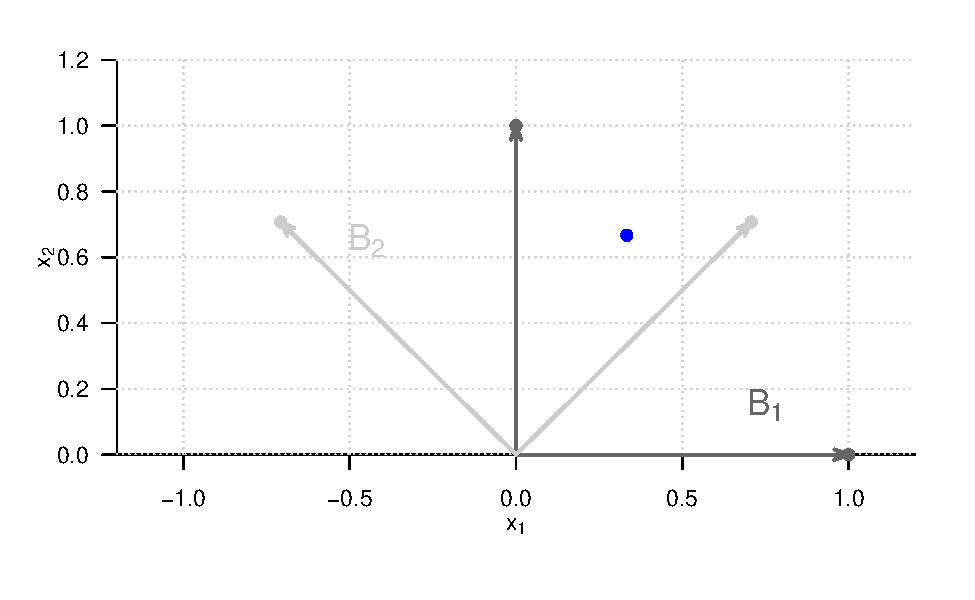
\includegraphics[width=0.7\linewidth]{4_Abbildungen/mvda_4_basen_R2} \end{center}

\small

Bei Hauptkomponenten- und Faktorenanalysen werden aus den Koordinaten
eines Vektors bezüglich einer Basis die Koordinaten desselben Vektors
bezüglich einer anderen Basis berechnet.
\end{frame}

\begin{frame}{Vektorkoordinatentransformation}
\protect\hypertarget{vektorkoordinatentransformation-1}{}
\small
\begin{definition}[Orthogonalprojektion]
$x$ und $q$ seien Vektoren im Euklidischen Vektorraum $\mathbb{R}^m$. Dann ist die
\textit{Orthogonalprojektion von $x$ auf $q$} definiert als der Vektor
\begin{equation}
\tilde{x} = aq \mbox{ mit } a := \frac{q^T x}{q^T q},
\end{equation}
wobei der Skalar $a$ \textit{Projektionsfaktor} genannt wird.
\end{definition}

\footnotesize

Bemerkungen

\begin{itemize}
\item Per definition ist  $\tilde{x} = aq$ mit $a \in \mathbb{R}$ der Punkt in Richtung von $q$ der $x$ am nähesten ist.
\item Diese minimierte Distanzeigenschaft impliziert die Orthogonalität von $q$ und $x - \tilde{x}$.
\item Die Formel von $a$ folgt direkt aus der Orthogonalität von $x - \tilde{x}$ und $q$, da gilt
\begin{equation*}
q^T(x - \tilde{x}) = 0
\Leftrightarrow
q^T(x - aq) = 0
\Leftrightarrow
q^Tx - aq^Tq = 0
\Leftrightarrow
a = \frac{q^Tx}{q^Tq}.
\end{equation*}
\item Wenn $q$ die Länge $||q|| = \sqrt{q^Tq} = 1$ hat, dann gilt $a = \frac{q^T x}{||q||^2} = q^T x$.
\end{itemize}
\end{frame}

\begin{frame}{Vektorkoordinatentransformation}
\protect\hypertarget{vektorkoordinatentransformation-2}{}
Orthogonalprojektion

\begin{center}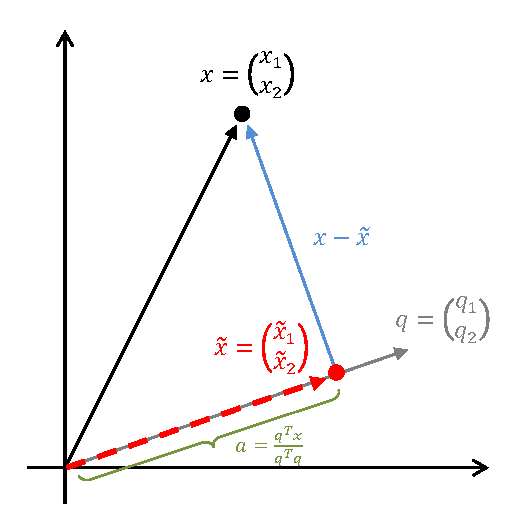
\includegraphics[width=0.6\linewidth]{4_Abbildungen/mvda_4_orthogonale_vektorprojektion} \end{center}
\end{frame}

\begin{frame}{Vektorkoordinatentransformation}
\protect\hypertarget{vektorkoordinatentransformation-3}{}
\footnotesize
\begin{theorem}[Vektorkoordinaten bezüglich einer Orthogonalbasis]
\justifying
\normalfont
Es sei $x \in \mathbb{R}^m$ und es sei $B := \{q_1,...,q_m\}$ eine Orthonormalbasis
von von $\mathbb{R}^m$. Dann ergeben sich für $i = 1,...,m$ die Koordinaten $a_i$ in
der Basisdarstellung von $x$ bezüglich $B$ als die Projektionsfaktoren
\begin{equation}
a_i = x^T q_i
\end{equation}
in der Orthogonalprojektion von $x$ auf $q_i$. Äquivalent ist die
Basisdarstellung von $x$ bezüglich $B$ gegeben durch
\begin{equation}
x = \sum_{i=1}^m (x^T q_i)q_i.
\end{equation}
\end{theorem}

\footnotesize

\underline{Beweis}

Für \(i = 1,...,m\) gilt \begin{equation}
x = \sum_{j=1}^m a_j q_j
\Leftrightarrow
q_i^T x = q_i^T \sum_{j=1}^m a_j q_j
\Leftrightarrow
q_i^T x = \sum_{j=1}^m a_j q_i^Tq_j
\Leftrightarrow
q_i^T x = a_i
\Leftrightarrow
a_i = x^T q_i.
\end{equation} \(\hfill \Box\)
\end{frame}

\begin{frame}{Vektorkoordinatentransformation}
\protect\hypertarget{vektorkoordinatentransformation-4}{}
\footnotesize
\begin{theorem}[Vektorkoordinatentransformation]
\justifying
\normalfont
$B_v := \{v_1,...,v_m\}$ und $B_w := \{w_1,...,w_m\}$ seien zwei Orthonormalbasen
eines Vektorraums. $A \in \mathbb{R}^{m \times m}$ sei die Matrix, die durch die
spaltenweise Konkatenation der Koordinaten der Vektoren in $B_w$ in der Basisdarstellung
bezüglich der Basis $B_v$ ergibt. Dann können die Koordinaten $x_i, i = 1,...,m$
eines Vektors $x$ bezüglich der Basis $B_v$ in die Koordinaten $\tilde{x}_1,...,\tilde{x}_m$
des Vektors bezüglich der Basis $B_w$  durch
\begin{equation}
\tilde{x} = A^T x
\end{equation}
transformiert werden. Analog können die Koordinaten $\tilde{y}_1,...,\tilde{y}_m$
des Vektors hinsichtlich der Basis $B_w$ in die Koordinaten $y_1,...,y_m$ des
Vektors hinsichtlich $B_v$ durch
\begin{equation}
x = A \tilde{x}.
\end{equation}
transformiert werden.
\end{theorem}

\footnotesize

Bemerkungen

\begin{itemize}
\tightlist
\item
  \justifying Das Theorem erlaubt die Berechnung von Vektorkoordinaten
  bezüglich einer anderen Orthonormalbasis.
\item
  Für die Berechnung muss zunächst die Matrix \(A\) gebildet und dann
  (nur) entsprechend multipliziert werden.
\item
  Wir verzichten auf einen Beweis und demonstrieren das Theorem an einem
  Beispiel.
\end{itemize}

\small
\center

\textcolor{darkblue}{Ein Vektor wird hier als  fester Punkt in $\mathbb{R}^m$ betrachtet; die Komponenten (Zahlen) des Vektors werden dagegen nur als Koordinaten bezüglich einer spezifischen Basis interpretiert!}
\end{frame}

\begin{frame}{Vektorkoordinatentransformation}
\protect\hypertarget{vektorkoordinatentransformation-5}{}
Beispiel \vspace{3mm}

\begin{center}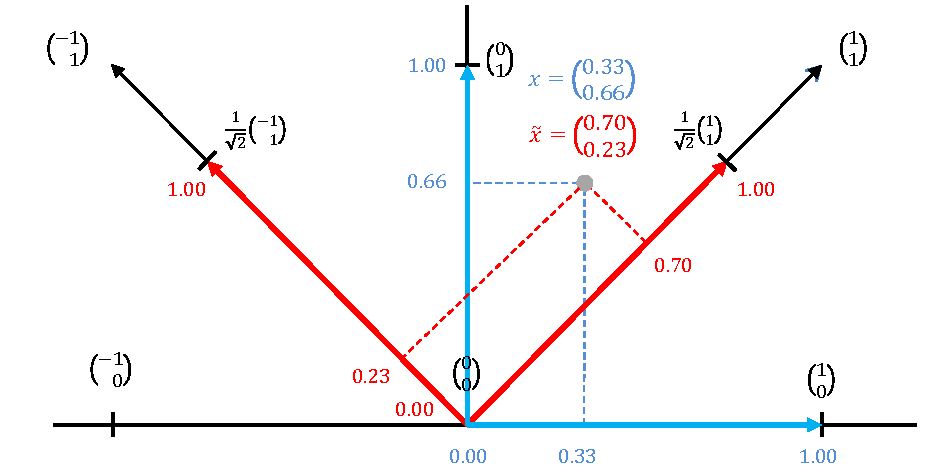
\includegraphics[width=1\linewidth]{4_Abbildungen/mvda_4_vektorkoordinatentransformation} \end{center}
\center
\vspace{1mm}
\small

Man beachte, dass \(x\) and \(\tilde{x}\) am selben Ort in
\(\mathbb{R}^2\) liegen!
\end{frame}

\begin{frame}{Vektorkoordinatentransformation}
\protect\hypertarget{vektorkoordinatentransformation-6}{}
\setstretch{1.2}
\vspace{2mm}

Beispiel \vspace{1mm}

\footnotesize

Wir nehmen an, dass wir die Koordinaten von
\(x = (1/3, 2/3)^T \in \mathbb{R}^2\) hinsichtlich der kanonischen
Orthonormalbasis \(B_v :=\{e_1,e_2\}\) in die Koordinaten bezüglich der
Basis \begin{equation}
B_w :=
\left\lbrace
\begin{pmatrix}
\frac{1}{\sqrt{2}} \\ \frac{1}{\sqrt{2}}
\end{pmatrix},
\begin{pmatrix}
-\frac{1}{\sqrt{2}} \\ \frac{1}{\sqrt{2}}
\end{pmatrix}
\right\rbrace
\end{equation} transformieren wollen. Die Basisdarstellungen der in
Vektoren \(B_w\) bezüglich der Basisvektoren in \(B_v\) sind
\begin{equation}
\begin{pmatrix}
\frac{1}{\sqrt{2}} \\ \frac{1}{\sqrt{2}}
\end{pmatrix}
=
a_{11}
\begin{pmatrix}
1 \\ 0
\end{pmatrix}
+
a_{21}
\begin{pmatrix}
0 \\ 1
\end{pmatrix}
\mbox{ and }
\begin{pmatrix}
-\frac{1}{\sqrt{2}} \\ \frac{1}{\sqrt{2}}
\end{pmatrix}
=
a_{12}
\begin{pmatrix}
1 \\ 0
\end{pmatrix}
+
a_{22}
\begin{pmatrix}
0 \\ 1
\end{pmatrix}.
\end{equation} Die Projektionsfaktoren der Orthogonalprojektionen der
Vektoren in \(B_w\) auf die Vektoren in \(B_v\) sind \begin{equation}
a_{11} =  \frac{1}{\sqrt{2}},
a_{21} =  \frac{1}{\sqrt{2}},
a_{12} = -\frac{1}{\sqrt{2}},
a_{22} =  \frac{1}{\sqrt{2}}.
\end{equation} Die Transformationsmatrix
\(A \in \mathbb{R}^{m \times m}\) in obigem Theorem ergibt sich also zu
\begin{equation}
A =
\begin{pmatrix}
a_{11} & a_{12} \\
a_{21} & a_{22} \\
\end{pmatrix}
=
\begin{pmatrix}
\frac{1}{\sqrt{2}} & -\frac{1}{\sqrt{2}} \\
\frac{1}{\sqrt{2}} &  \frac{1}{\sqrt{2}} \\
\end{pmatrix}.
\end{equation} Die Vektorkoordinatentransformation von
\(x \in \mathbb{R}^2\) ergibt sich also zu \begin{equation}
\tilde{x}
= A^T x
= \begin{pmatrix}
\frac{1}{\sqrt{2}} & \frac{1}{\sqrt{2}}     \\
-\frac{1}{\sqrt{2}} &  \frac{1}{\sqrt{2}}   \\
\end{pmatrix}
\begin{pmatrix}
\frac{1}{3} \\
\frac{2}{3}
\end{pmatrix}
\approx
\begin{pmatrix}
0.70 \\
0.23
\end{pmatrix}.
\end{equation}
\end{frame}

\begin{frame}{}
\protect\hypertarget{section-7}{}
\vfill
\setstretch{2.5}
\Large

Eigenvektoren und Eigenwerte

Orthonormalzerlegung

Singulärwertzerlegung

Vektorkoordinatentransformation

\textbf{Selbstkontrollfragen} \vfill 
\end{frame}

\begin{frame}{Selbstkontrollfragen}
\protect\hypertarget{selbstkontrollfragen}{}
\footnotesize
\setstretch{2}
\begin{enumerate}
\item Geben Sie die Definition eines Eigenvektors und eines Eigenwertes einer quadratischen Matrix wieder.
\item Geben Sie das Theorem zur Bestimmung von Eigenwerten und Eigenvektoren wieder.
\item Geben Sie das Theorem zu den Eigenwerten und Eigenvektoren symmetrischer Matrizen wieder.
\item Geben Sie das Theorem zur orthonormalen Zerlegung einer symmetrischen Matrix wieder.
\item Geben Sie die Definition einer Singulärwertzerlegung wieder.
\item Geben Sie das Theorem zum Zusammenhang von Singulärwertzerlegung und Eigenanalyse wieder.
\item Definieren Sie den Begriff Orthogonalprojektion.
\item Geben Sie das Theorem zu Vektorkoordinaten bezüglich einer Orthogonalbasis wieder.
\item Geben Sie das Vektorkoordinatentransformationstheorem wieder.
\item Erläutern Sie das Vektorkoordinatentransformationstheorem.
\end{enumerate}
\end{frame}

\begin{frame}{References}
\protect\hypertarget{references}{}
\footnotesize

\hypertarget{refs}{}
\begin{CSLReferences}{1}{0}
\leavevmode\vadjust pre{\hypertarget{ref-strang_2009}{}}%
Strang, Gilbert. 2009. \emph{Introduction to {Linear Algebra}}.

\end{CSLReferences}
\end{frame}

\end{document}
